\documentclass[10pt]{exam}
\usepackage[phy]{template-for-exam}
\usepackage{silence,tikz,multicol}
\WarningFilter{latex}{Label `question}
\WarningFilter{latex}{There were multiply-defined labels}

\title{Sound Stations}
\author{Rohrbach}
\date{\today}

\begin{document}
\maketitle

\section{Section 20.1 : The Nature of Sound}

Read Section 20.1 (pp. 375-376)

\begin{questions}
  \question 
    How are sound waves produced?

  \question 
    What type of wave is a sound wave?

  \question 
    Define the following terms:

    \begin{parts}
      \part pitch
      \part infrasonic
      \part ultrasonic
    \end{parts}

  \question 
    What sorts of materials cause sound to travel more quickly?  Why?

\end{questions}

\section{Function Generator and Speaker}

\begin{questions}
  \question
    Adjust the frequency and the amplitude.  Describe what you notice about the sound.

  \question
    Start the frequency very low (2 Hz or smaller).  Slowly increase the frequency until it starts to sound like a tone.  This is the point at which the sound stops being \emph{infrasonic}.  Write down this frequency.


  \question
    Start the frequency very high (Above 40,000 Hz).  Slowly decrease the frequency until you can hear it.  This is the point at which the sound stops being \emph{ultrasonic}.  Write down this frequency.  When you are finished, {\bf please make sure to turn the amplitude all the way down so it doesn't bother your classmates}.

\end{questions}

\section{Sections 20.5-20.6 : Forced Vibrations and Resonance}

Read Sections 20.5 and 20.6 (pp. 382-383)

\begin{questions}
  \label{resonance}

  \question
    Define the following terms:

    \begin{parts}
      \part forced vibration
      \part natural frequency  
      \part resonance
    \end{parts}

  \question
    Explain how resonance relates to a kid on a swing.

  \question
    Make your own sounding board!  Hit a tuning fork against the table.  Then place it stem-side down on the table and listen to what happens.  Use your definition for ``force vibration'' above to explain what is happening here.
  
\end{questions}

\section{Resonance Tube}

\begin{questions}
  \question
    Hit the tuning fork against the table to generate a tone.  Hold it over the resonance tube.  Keep changing the length of the resonance tube until you hear the sound get louder.  What is happening and why?

  \question
    Look at your definitions from Station~\ref{resonance}.  What do you think you are changing when you change the length of the tube?

  \question
    Now, turn on the function generator.  Gradually change the frequency.  Pay attention to what happens to each of the three metal sheets.  Explain why you think that they don't all resonate at the same time.
    
\end{questions}



\section{Generating Acoustic Beats}

  You will define the term ``acoustic beats'' at the next station.  But, in the meantime, let's experience what beats are.

  \begin{questions}
    \question
      There are two tuning forks in front of you.  One has adjustable weights.  Make sure each of the weights is lined up with the indented line on the tuning fork.  Hit each tuning fork.  They should sound the same.
    \question
      Now, change the frequency of the adjustable tuning fork slightly by lowering one of the weights by 1-2 centimeters.  Play both tuning forks again.  Explain what you are hearing.  
    \question
      This ``throbbing'' or ``wobbling'' you are hearing is called ``acoustic beats.'' Move the weight even further and play the tuning forks.  You should notice that the ``throbbing'' changes frequency.  Does it shift to a higher frequency or a lower frequency?

    \question
      To explain why beats occur, take a look at the two pendulums hanging at your station.  They are different lengths, which means they have different periods and different frequencies.  Set them both in motion and watch what happens.  Do they ever look like they are in sync?  Do they ever look like they're out of sync?
  \end{questions}
 
\section{Section 20.8 : Beats}

Read Section 20.8 (pp. 385-386)

\begin{questions}
  \question
    What are ``\emph{beats}''?

  \question
    In experiencing beats, why does the sound switch from loud to soft to loud to soft?

  \question
    Look at the diagram below (Figure 20.21 from the textbook).  Label the regions of constructive and destructive interference.

    \begin{tikzpicture}
      \node at (0,0) 
        {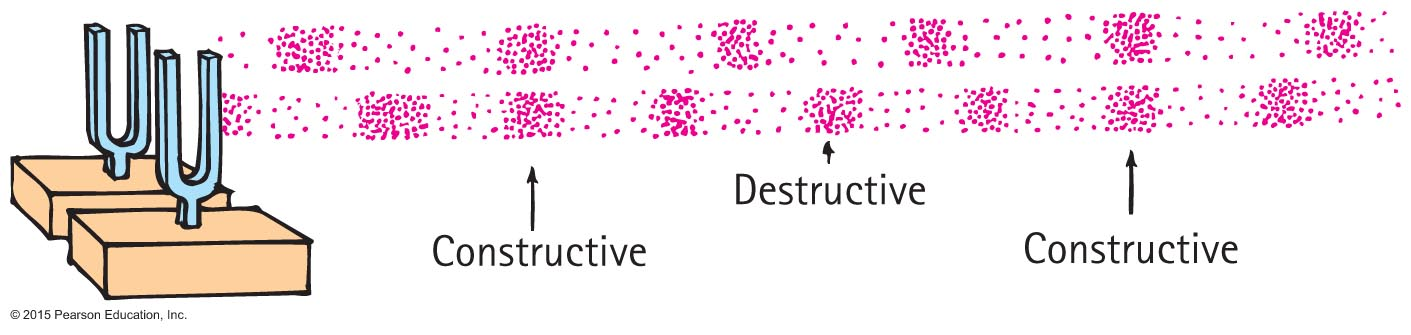
\includegraphics[width=12cm]{Fig20_21.jpg}};
      \fill[white] (-3,-1) rectangle (6,.26);
    \end{tikzpicture}
 
  \question
    Draw your own beats!  Draw two bunnies hopping forward.  One bunny jumps forward 3 cm each hop; the other bunny jumps forward 4 cm each hop.  Circle the locations where the bunnies are `'`in sync.''

    \begin{tikzpicture}
      \draw[dotted] (0,0) grid[step=0.5] (15,-1.5);
      \fill (0,-0.5) circle (0.1)
        ++ (1.5,0) circle (0.1)
        ++ (1.5,0) circle (0.1);
      \fill (0,-1) circle (0.1)
        ++ (2,0) circle (0.1)
        ++ (2,0) circle (0.1);
    \end{tikzpicture}
\end{questions}

\section{}

\section{}

\end{document}